% Created 2017-08-14 Mon 11:07
\documentclass[11pt]{article}
\usepackage[utf8]{inputenc}
\usepackage[T1]{fontenc}
\usepackage{fixltx2e}
\usepackage{graphicx}
\usepackage{grffile}
\usepackage{longtable}
\usepackage{wrapfig}
\usepackage{rotating}
\usepackage[normalem]{ulem}
\usepackage{amsmath}
\usepackage{textcomp}
\usepackage{amssymb}
\usepackage{capt-of}
\usepackage{hyperref}
\usepackage{graphicx}
\graphicspath{ {assets/} }
\author{DESKTOP-RI55L4A}
\date{\today}
\title{}
\hypersetup{
 pdfauthor={DESKTOP-RI55L4A},
 pdftitle={},
 pdfkeywords={},
 pdfsubject={},
 pdfcreator={Emacs 25.2.50.1 (Org mode 8.3.5)}, 
 pdflang={English}}
\begin{document}

\tableofcontents


\section{Evaluation}
\label{sec:orgheadline5}
\subsection{Introduction}
\label{sec:orgheadline1}
\subsection{Initial pilot test}
\label{sec:orgheadline2}
\begin{description}
\item[{Introduction}] Describe methodology used
\item Describe results
\item Describe comments and feedback
\item Verified that it was approachable and basically worked as a NUI application
\end{description}
\subsection{Exhibition}
\label{sec:orgheadline3}

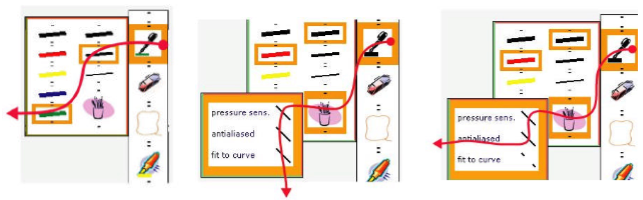
\includegraphics{crossy.png}

\subsection{Conclusion}
\label{sec:orgheadline4}
\end{document}